\documentclass[10pt,a4paper]{article}
\usepackage[utf8]{inputenc}
\usepackage[T1]{fontenc}
\usepackage{amsmath}
\usepackage{amsfonts}
\usepackage{amssymb}
\usepackage{graphicx}
\usepackage{listings}
\usepackage{float}
\usepackage{multirow}
\usepackage{subcaption}
\usepackage[table]{xcolor}
\usepackage[labelformat=parens,labelsep=quad,skip=3pt]{caption}


\begin{document}
	\title{Homework 5 -I2C EEPROM}
	\makeatletter
	
	\author{Zackary McClamma\thanks{University of Dayton}
		\thanks{Dept. of Electrical and Computer
			Engineering, University of Dayton, 300 College Park, Dayton, OH
			45469-0226, U.S.A. E-mail:
			mcclammaz1@udayton.edu}}
	
	\makeatother
	
	\date{\today}
	
	\maketitle
	\section{Introduction}
	This homework assignment was focused on resource sharing and consisted of running the $\mu$C/OS-II\texttrademark operating system with two tasks, a mutex, and an EEPROM read and write function. The first task consists of displaying a menu in the terminal with four options, Write EEPROM, Read EEPROM, Red LED on, and Red LED off. The second task toggles a green LED on and off, changing the state of the LED every 500ms.
	
	\section{System Design}
 	This system uses i2c communications to read and write to an EEPROM device on the board. The options for telling the OS what to do are selected by a user by using the menu displayed in the terminal. The system includes the Nios II processor, an I2C controller, on-chip memory (RAM), and two peripherals a red LED and a green LED. In contrast to the last assignment where we created our own print function, in this assignment we will be using printf and scanf to read from and write to the terminal. 

	
	\section{Theory of Operation}
	In this system the majority of the work is done in software since the only peripherals I2C controller, the LEDs, and the clock. The Nios-II processor is first loaded onto the FPGA along with the memory. The operating system is then loaded onto the processor and is used to create two tasks. The first task prints menu where a user can select from four options. The first option is "Write EEPROM if the user selects this option they will be prompted for an address to write to and the data they want to write. The second option is "Read EEPROM" when this is selected the user will be prompted for an address and the program will return the data at that location. Options 3 and 4 are "Turn on Red LED" and "Turn off Red LED" respectively, as the menu choices indicate these will turn the Red LED on or off. A diagram of the functioning system can be seen in Figure \ref{block} 
	\begin{figure}[H]
		\centering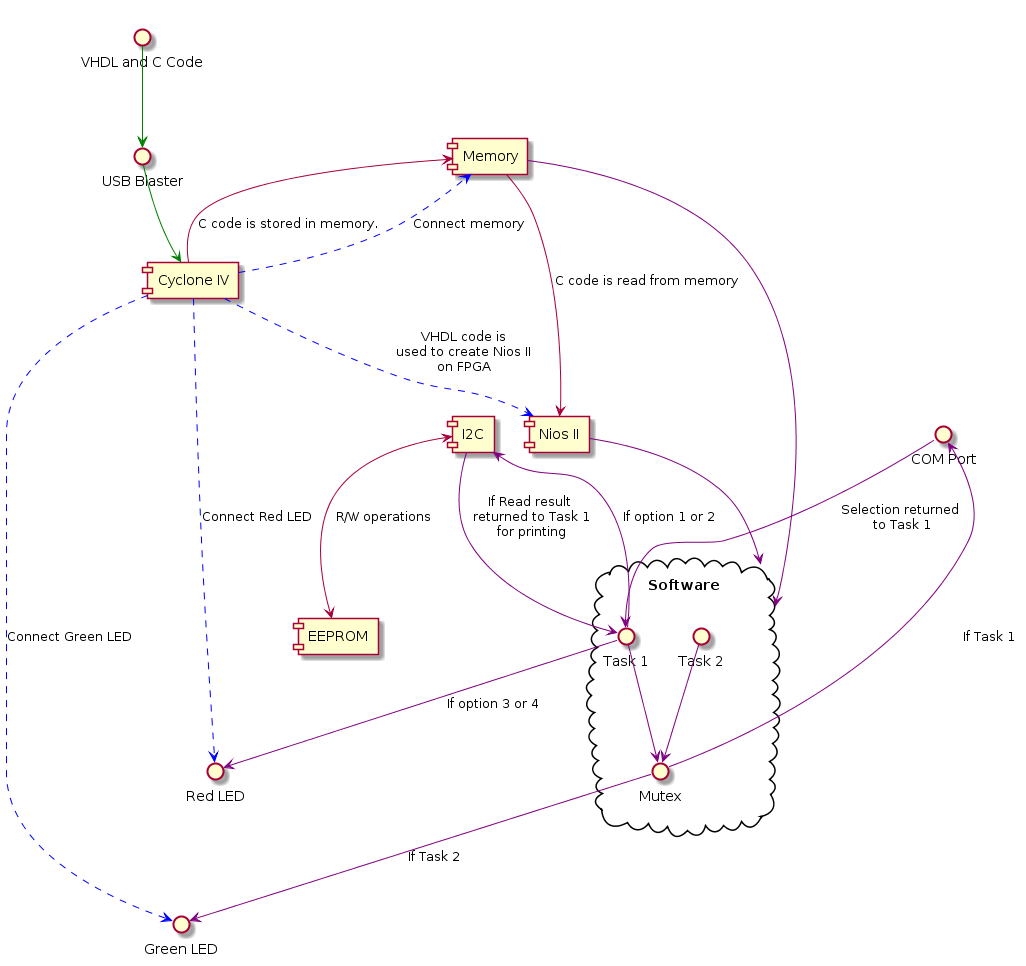
\includegraphics[height=15cm]{HW5_Block.png}
		\caption{Embedded System Block Diagram}
		\label{block}
	\end{figure}


	\section{Results}
	I was able to get everything to work correctly except the tasking, for some reason every time that I generated the hello\_uosii program there was an error in "hw5\_bsp/HAL/src/os\_cpu\_c.c" in the OSTaskHook function. I attempted to regenerate multiple times and every time it produced the same file and the file would not show an error when building but as soon as I would run the program the error would be there even though I verified the file was the same as before I ran my program. For this reason both tasks wouldn't run at the same time, the program would only run whichever program I put at a higher priority. I am not sure why it happened with this assignment and no the last one. Below is an image of the terminal output for the EEPROM. I can demonstrate the LED functionality in class if needed.
	
	\begin{figure}[H]
		\centering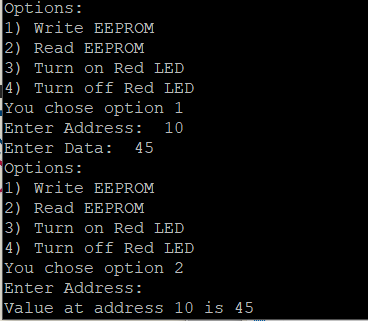
\includegraphics[width=10cm]{EEPROM_Term_Output.png}
		\caption{Terminal output of EEPROM Read and Write}
		\label{tex}
	\end{figure}

	\section{Conclusion}
	This homework assignment took me to the last minute to complete because of an oversight on my part. I neglected to assign pins to the i2c clock and data and it took me until a few hours before the assignment was due to realize it. Other than that the i2c was a bit confusing to figure out but once I was able to tackle that and actually able to troubleshoot it, the rest of the assignment was pretty easy.
	
	\clearpage
	\appendix
	\section{\\VHDL Code}
	\lstinputlisting[language=VHDL]{homework5.vhd}
	
	\section{\\C Code}
	\subsection{Headers}
	\lstinputlisting[language=C]{hw5.h}
	
	\subsection{Source}
	\lstinputlisting[language=C]{main.c}
\end{document}